\section{Introduction}
\label{sec:intro}

Language models are increasingly deployed as agents for planning, tool use, and environment interaction~\citep{gao2025survey, hu2026owl, luo2025large, luo2025agentmath, zhou2026offseeker}. On-policy distillation (OPD) offers a promising training framework for such agentic models~\citep{lu2025onpolicydistillation, li2026rethinking}, where a student samples rollouts and a stronger teacher supervises via a reverse-KL objective at visited states. This keeps supervision on-policy and provides dense feedback while avoiding sparse reward signals.

Yet, applying OPD to long-horizon agent tasks is challenging because these are more than simple sequence-generation problems~\citep{zhong2026sod,wang2026tcod}. Agent rollouts involve multiple turns, tool calls, environmental shifts, and state changes. Early decisions impact all subsequent states, and later turns often contain key but infrequent decisions, so token-level feedback alone may not provide proper supervision for all crucial points.

\begin{figure}[t]
\centering
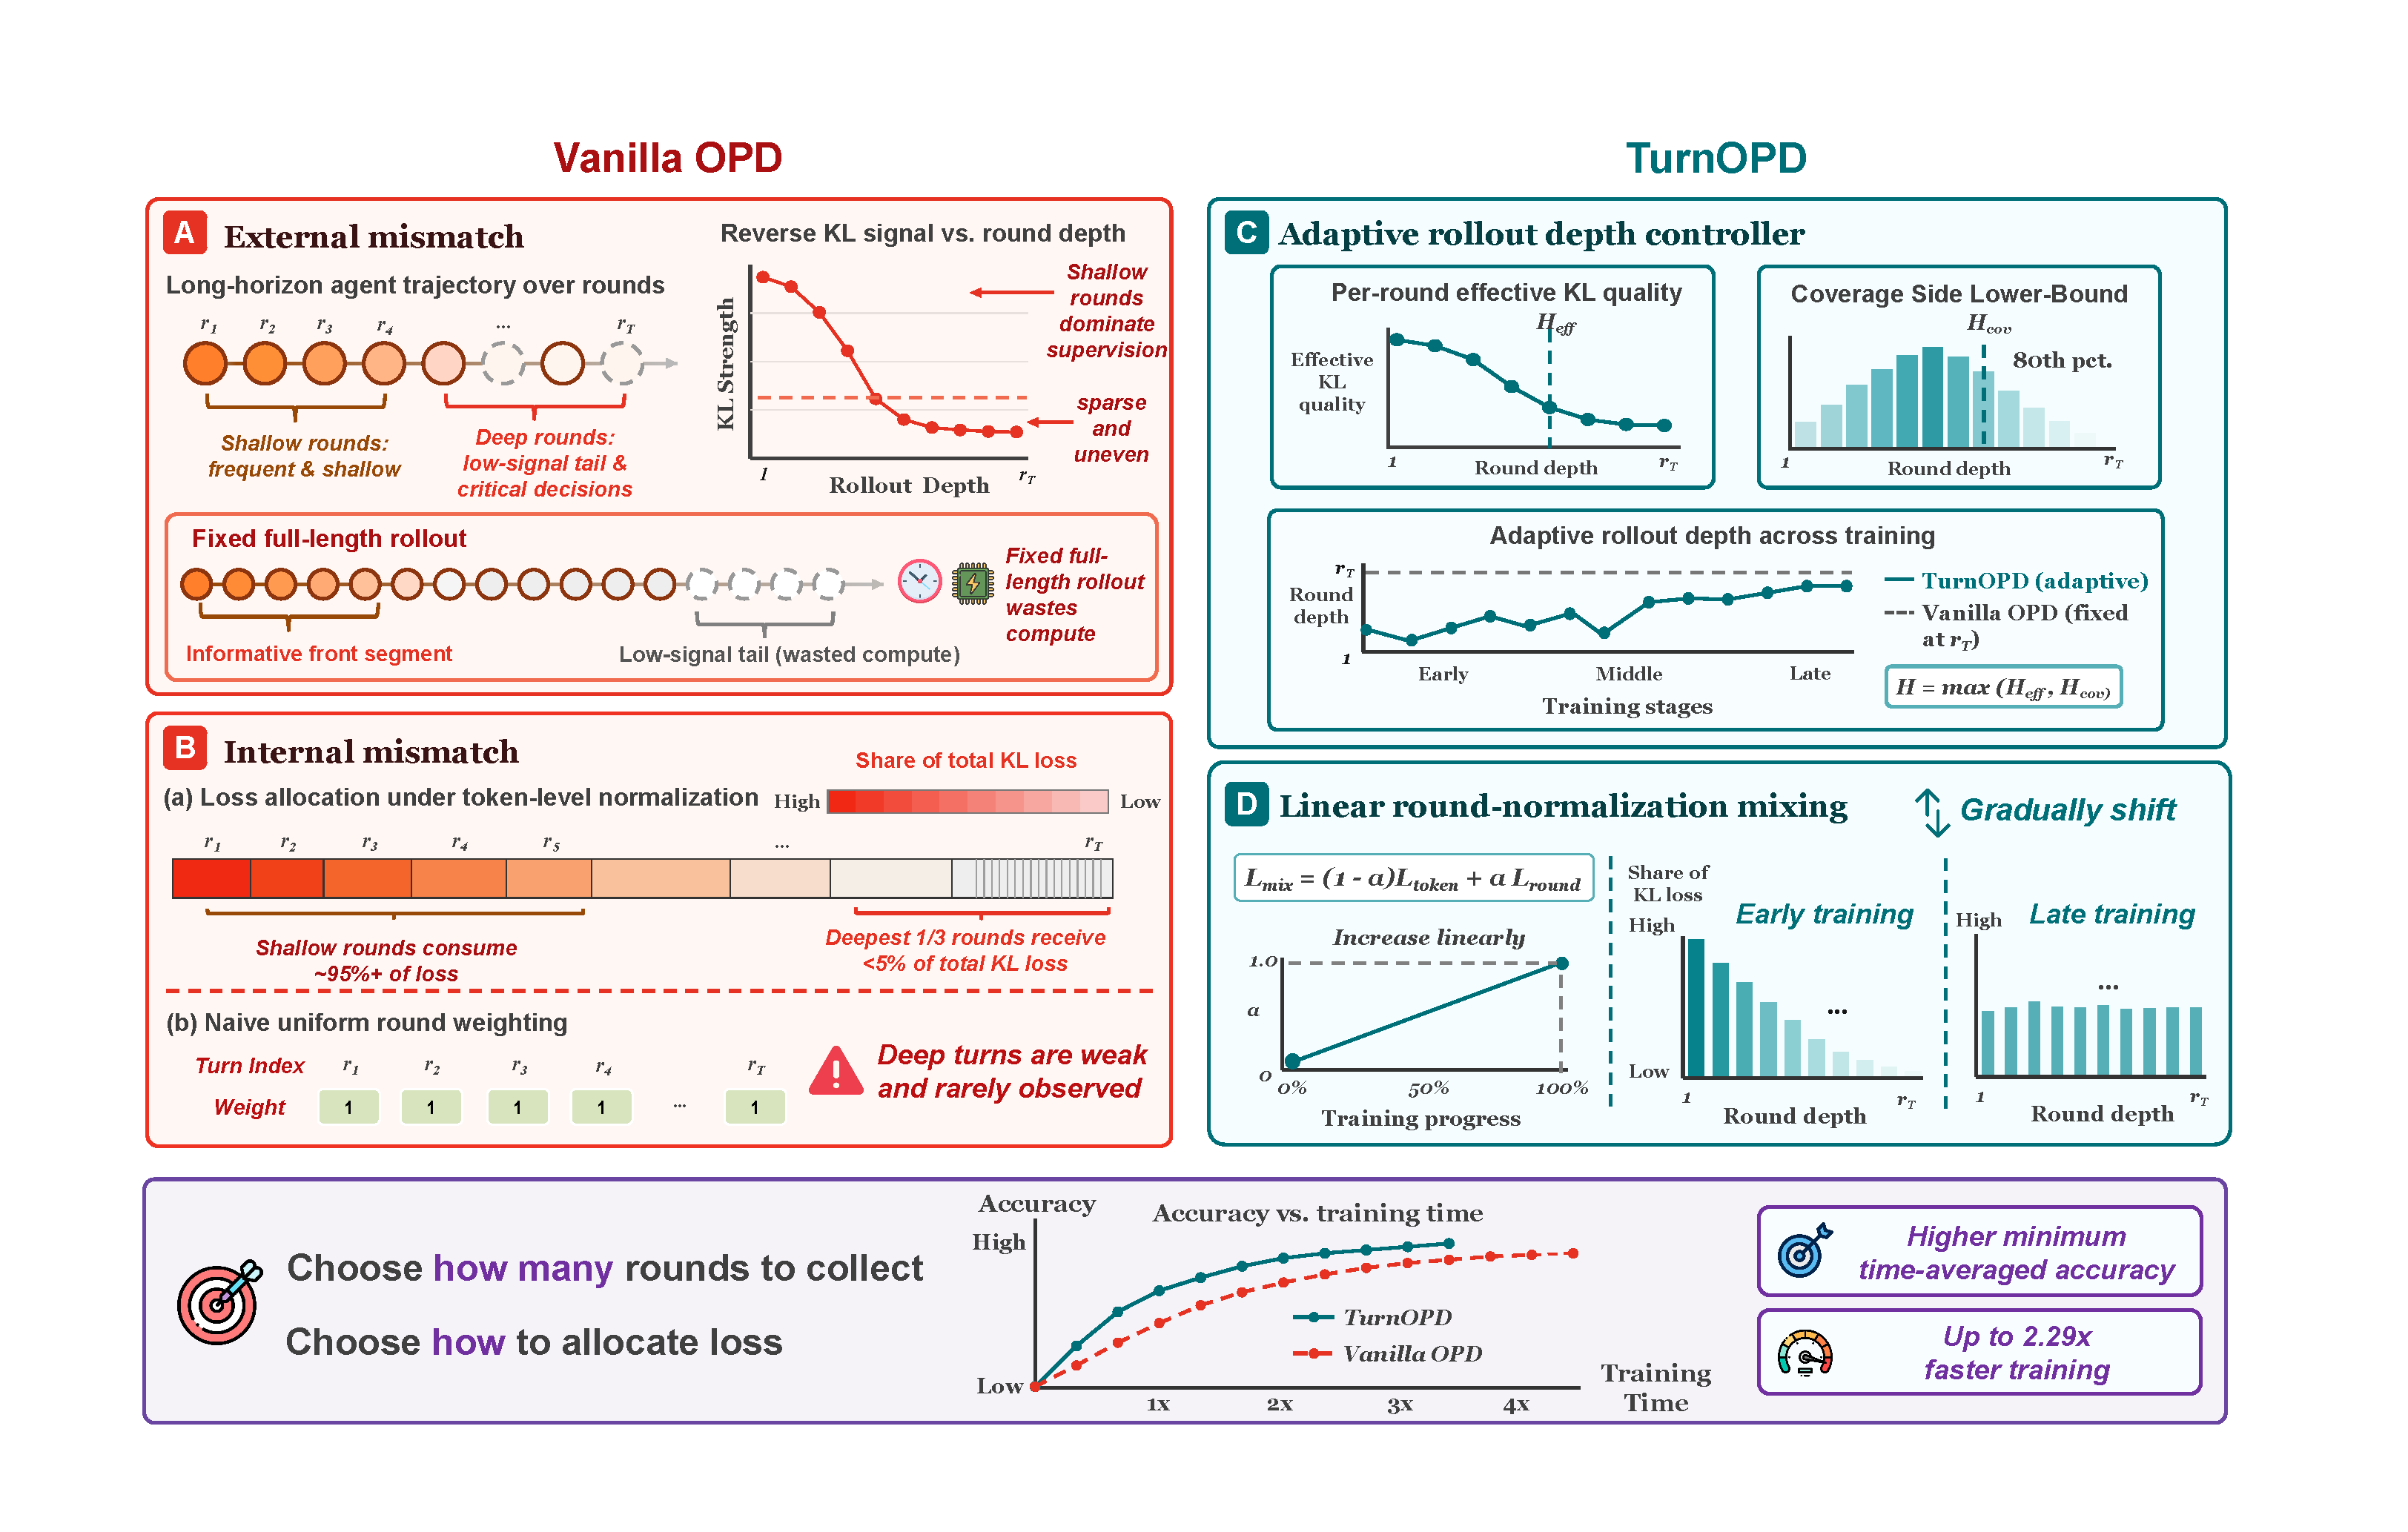
\includegraphics[width=0.98\linewidth]{figures/TurnOPD_introduction.pdf}
\caption{A turn-aware perspective on agent OPD. Standard OPD fixes the rollout depth and averages KL across the full trajectory, often wasting resources on low-value tail turns and over-focusing loss on shallow tokens. TurnOPD budgets both rollout depth and KL aggregation based on turn-level statistics, providing a more balanced supervision signal.}
\label{fig:intro-tasc-overview}
\vspace{-0.3cm}
\end{figure}

We systematically analyze OPD in long-horizon agent tasks, asking: \textit{How are supervision signals and optimization budgets allocated along the interaction trajectory, and with what consequences?} Our diagnosis identifies two main problems: \textbf{(1) Per-turn KL distribution:} The reverse-KL signal is heavily skewed toward early turns, changes over training, and becomes less informative for deeper steps. Student and teacher outputs often converge as more context is self-generated, reducing observed KL even when meaningful disagreements persist. \textbf{(2) Loss budget:} The optimizer's loss is not equitably distributed—shallow turns are overrepresented and carry higher KL, so they dominate the loss, while deep turns contribute little. For example, only $3.6$--$4.5\%$ of the KL loss is assigned to the deepest third of turns on ALFWorld~\citep{shridhar2021alfworld}, and $11$--$13\%$ on Multi-Hop Search. While strict turn-level normalization can mitigate this, it risks over-weighting deep, low-data turns. Overall, standard KL supervision and normalization along full trajectories are insufficient.

These issues stem from two mismatches: (1) \textbf{External mismatch:} Fixed rollout depth ignores that both correction signal and survivor count vary markedly with turn. Expending compute up to the maximum horizon wastes effort on steps with little reliable signal. (2) \textbf{Internal mismatch:} Trajectory-level normalization gives uniform token weights, concentrating the KL signal on easy, shallow turns and starving deep, informative ones once the model learns basic interaction patterns.

To address these, we propose \textbf{TurnOPD}, a turn-level budgeting strategy for efficient on-policy distillation of long-horizon agents. TurnOPD consists of two budget controllers. The \textbf{adaptive rollout-depth} controller dynamically selects rollout length via periodic probes, guided by survivor-weighted KL and coverage thresholds. The \textbf{progressive turn-normalized loss} controller gradually transitions KL loss aggregation from trajectory-level to turn-balanced, increasing the weight of deep turns.

We evaluate TurnOPD on three representative multi-turn agent benchmarks: embodied planning (ALFWorld), web navigation (WebShop)~\citep{yao2022webshop}, and Multi-Hop Search (including PopQA~\citep{mallen2023popqa}, NQ~\citep{kwiatkowski2019natural}, 2WikiMultiHopQA~\citep{ho2020twowiki}, HotpotQA~\citep{yang2018hotpotqa}). TurnOPD improves minimal-time Avg@4 across all tasks and models. For example, on ALFWorld-1.7B, it increases Same-Step Avg@4 from $83.0$ to $86.3$ and cuts 100-step wall time from $4.42$h to $1.93$h. On WebShop, both accuracy and wall time (from $1.57$h to $1.24$h) are improved.
Our ablations further support the decomposition. Adaptive depth is the main efficiency lever: on ALFWorld-1.7B, it nearly halves wall time but does not by itself solve the loss-allocation problem, while linear KL blending improves Same-Step Avg@4 by reallocating supervision toward deeper turns. Combining both gives the best accuracy--time tradeoff, and coverage-floor studies show that the controller can be tuned smoothly between conservative and aggressive rollout horizons.

In summary, our contributions are as follows:
\begin{itemize}[leftmargin=1.5em,itemsep=2pt,topsep=3pt]
\item We provide a turn-level analysis of OPD for long-horizon agents, revealing the general distribution of supervision and optimization signals across decision turns.
\item We formalize one contamination-compression mechanism for the mismatch phenomenon of OPD in long-horizon agent tasks, and demonstrate the existence of a potentially optimal rollout horizon.
\item We propose \textbf{TurnOPD}, which combines adaptive rollout-depth budgeting with progressive turn-normalized loss budgeting.
\item We demonstrate that TurnOPD achieves the best Least-Time accuracy on tested benchmarks, advancing the accuracy--time frontier. Notably, TurnOPD achieves comparable or even better performance with up to 2.29$\times$ faster training.
\end{itemize}
